%!TeX root=../tese.tex
\chapter{Grau limitado}
\label{cap:grau-limitado}

% ---------------------------------------
% ------- Vibe coding começa aqui -------
% ---------------------------------------

% Comando personalizado para desenhar o grafo de Andrásfai com parâmetro d
\newcommand{\drawAndrasfai}[1]{%
  \def\d{#1}                              % parâmetro d
  \pgfmathsetmacro\n{int(3*\d - 1)}       % número de vértices n = 3d - 2
  \begin{tikzpicture}[scale=1.5,
    every node/.style={circle, draw, fill=white, inner sep=1pt, font=\small}]
  
  % 1. Coloca os vértices uniformemente em círculo
  \foreach \i in {0,...,\numexpr \n-1 \relax} {
    \pgfmathsetmacro\angle{90-360*\i/\n}
    \node (v\i) at (\angle:1) {\i};       % vértice v_i na posição angular correspondente
  }

  % 2. Para cada vértice, conecta aos d vértices mais distantes
  \foreach \i in {0,...,\numexpr \n-1 \relax} {
    \foreach \offset in {0,...,\numexpr \d-1 \relax} {
      \pgfmathsetmacro\j{mod(\i + \d + \offset, \n)} % vértice mais distante no ciclo
      \pgfmathtruncatemacro{\ii}{\i}
      \pgfmathtruncatemacro{\jj}{\j}
      \ifnum\ii<\jj
        \draw (v\ii) -- (v\jj);          % desenha aresta se ii < jj (para evitar duplicação)
      \fi
    }
  }

  \end{tikzpicture}
}

% --------------------------------------
% ------ Vibe coding termina aqui ------
% --------------------------------------

\newcommand{\homarrow}{\xhookrightarrow{\text{hom}}}

Vamos tentar resolver quando $\delta(G)$ é grande?
Ok, ok, você vai dizer ``mas o resultado do capítulo 2 já cobre isso''.
Verdade, mas queremos mais \textit{estrutura} sobre os conjuntos que geram $D(G)$, então ainda vale a pena estudar esses casos!

Seja $d \geq 1$ um inteiro positivo.

\begin{definition}
  Seja $d \geq 1$ um inteiro positivo.
  O \emph{grafo de Andrásfai} $F_d$ é o grafo com vértices $\{0,1,\dots,3d-2\}$ e arestas entre $i$ e $i+d+j$ para cada $j \in \{0,1,\dots,d-1\}$.
  Uma forma de representar os grafos de Andrásfai é colocar os vértices em uma circunferência em sentido horário como vértices de $(3d-1)$-ágono regular e ligar cada vértice com os $d$ vértices mais distantes dele.

  \begin{figure}[htbp]
    \centering

    \begin{subfigure}[b]{0.22\textwidth}
      \centering
      \drawAndrasfai{1}
      \caption*{$F_1$}
    \end{subfigure}
    \hfill
    \begin{subfigure}[b]{0.22\textwidth}
      \centering
      \drawAndrasfai{2}
      \caption*{$F_2$}
    \end{subfigure}
    \hfill
    \begin{subfigure}[b]{0.22\textwidth}
      \centering
      \drawAndrasfai{3}
      \caption*{$F_3$}
    \end{subfigure}
    \hfill
    \begin{subfigure}[b]{0.22\textwidth}
      \centering
      \drawAndrasfai{4}
      \caption*{$F_4$}
    \end{subfigure}

    \caption{Grafos de Andrásfai para $d = 1$ a $d = 4$. Observe que $F_d$ é $d$-regular e livre de triângulos.}
  \end{figure}
\end{definition}

\begin{theorem} [\cite{jin199510n29}] \label{thm:jin}
  Seja $G$ um grafo livre de triângulos com $n$ vértices e grau mínimo maior que $10n/29$.
  Então $G \homarrow F_9$.
\end{theorem}

\begin{theorem} [\cite{chen1997triangle}] \label{thm:hom-to-Fd}
  Seja $G$ um grafo livre de triângulos com $n$ vértices e $\chi(G) \leq 3$.
  Se $\delta(G) > \frac{d+1}{3d+2}n$, então $G$ está contido em um blow-up de $F_d$.
\end{theorem}

\begin{lemma} \label{lem:odd-transversal}
  Seja $G$ um grafo e suponha que existem conjuntos dois a dois disjuntos $E_1,E_2,E_3,E_4,E_5 \subseteq E$ tais que
  $G-F_i$ é bipartido para cada $i \in \{1,2,3,4,5\}$.
  Então $G$ satisfaz a Conjectura \ref{conj:make-bipartite}.
\end{lemma}

\begin{proof}
  Se $e(G) \geq \frac{n^2}{5}$, então o resultado segue do Teorema \ref{thm:n2/5}.
  Por outro lado, se $e(G) < \frac{n^2}{5}$, então
    \[ 5 \min\{ |E_1|,|E_2|,|E_3|,|E_4|,|E_5| \} \leq |E_1|+|E_2|+|E_3|+|E_4|+|E_5| \leq e(G) < \frac{n^2}{5}, \]
  de forma que para $|E_i| = \min \{ |E_1|,|E_2|,|E_3|,|E_4|,|E_5| \}$ temos $G-E_i$ bipartido com $|E_i| < \frac{n^2}{25}$.
\end{proof}

Esse Lema vai funcionar para $F_4$, mas não para $F_5$.

\begin{theorem}
  Se $G$ é um grafo livre de triângulo com $n$ vértices e $\delta(G) > 4n/11$, então $D(G) \leq \frac{n^2}{25}$.
\end{theorem}

\begin{proof}
  Veja que $4/11 > 10/29$, logo pelo Teorema \ref{thm:jin}, temos que $G \homarrow F_9$.
  Em particular, $\chi(G) \leq \chi(F_9) = 3$.
  Assim, pelo Teorema \ref{thm:hom-to-Fd} com $d=3$, vale que $G \homarrow F_4$.
  Considere a seguinte partição das arestas de $G$, em que cada classe está representada por um vértice e todos as arestas entre o mesmo par de classes estão na mesma parte:

  \begin{center}
    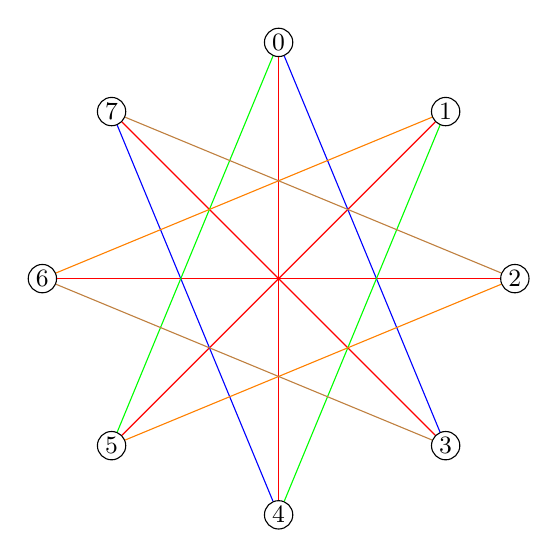
\begin{tikzpicture}[scale=3,
      every node/.style={circle, draw, fill=white, inner sep=1pt, font=\small}]
    
    % 1. Coloca os vértices uniformemente em círculo
    \foreach \i in {0,...,7} {
      \pgfmathsetmacro\angle{90-360*\i/8}
      \node (v\i) at (\angle:1) {\i};       % vértice v_i na posição angular correspondente
    }

    \draw [red] (v0)--(v4);
    \draw [red] (v1)--(v5);
    \draw [red] (v2)--(v6);
    \draw [red] (v3)--(v7);

    \draw [blue] (v0)--(v3);
    \draw [blue] (v7)--(v4);

    \draw [green] (v1)--(v4);
    \draw [green] (v0)--(v5);

    \draw [orange] (v1)--(v6);
    \draw [orange] (v2)--(v5);

    \draw [brown] (v3)--(v6);
    \draw [brown] (v2)--(v7);

    \end{tikzpicture}
  \end{center}

  Como a remoção de cada uma das partes deixa $G$ bipartido, podemos aplicar o Lema \ref{lem:odd-transversal} a $G$.
  Isso conclui a prova do Teorema. 
\end{proof}
